\documentclass{beamer}

\usetheme{CambridgeUS}
\usecolortheme{beaver}
\usefonttheme{professionalfonts}
\setbeamertemplate{blocks}[rounded][shadow]
\setbeamertemplate{title page}[default][colsep=-4bp,rounded=true]

\beamertemplatenavigationsymbolsempty

\usepackage[english]{babel}

\usepackage{amssymb}

\graphicspath{{images/}}

\title{XY model}
\date{}

\begin{document}

\begin{frame}[plain]

\begin{center}
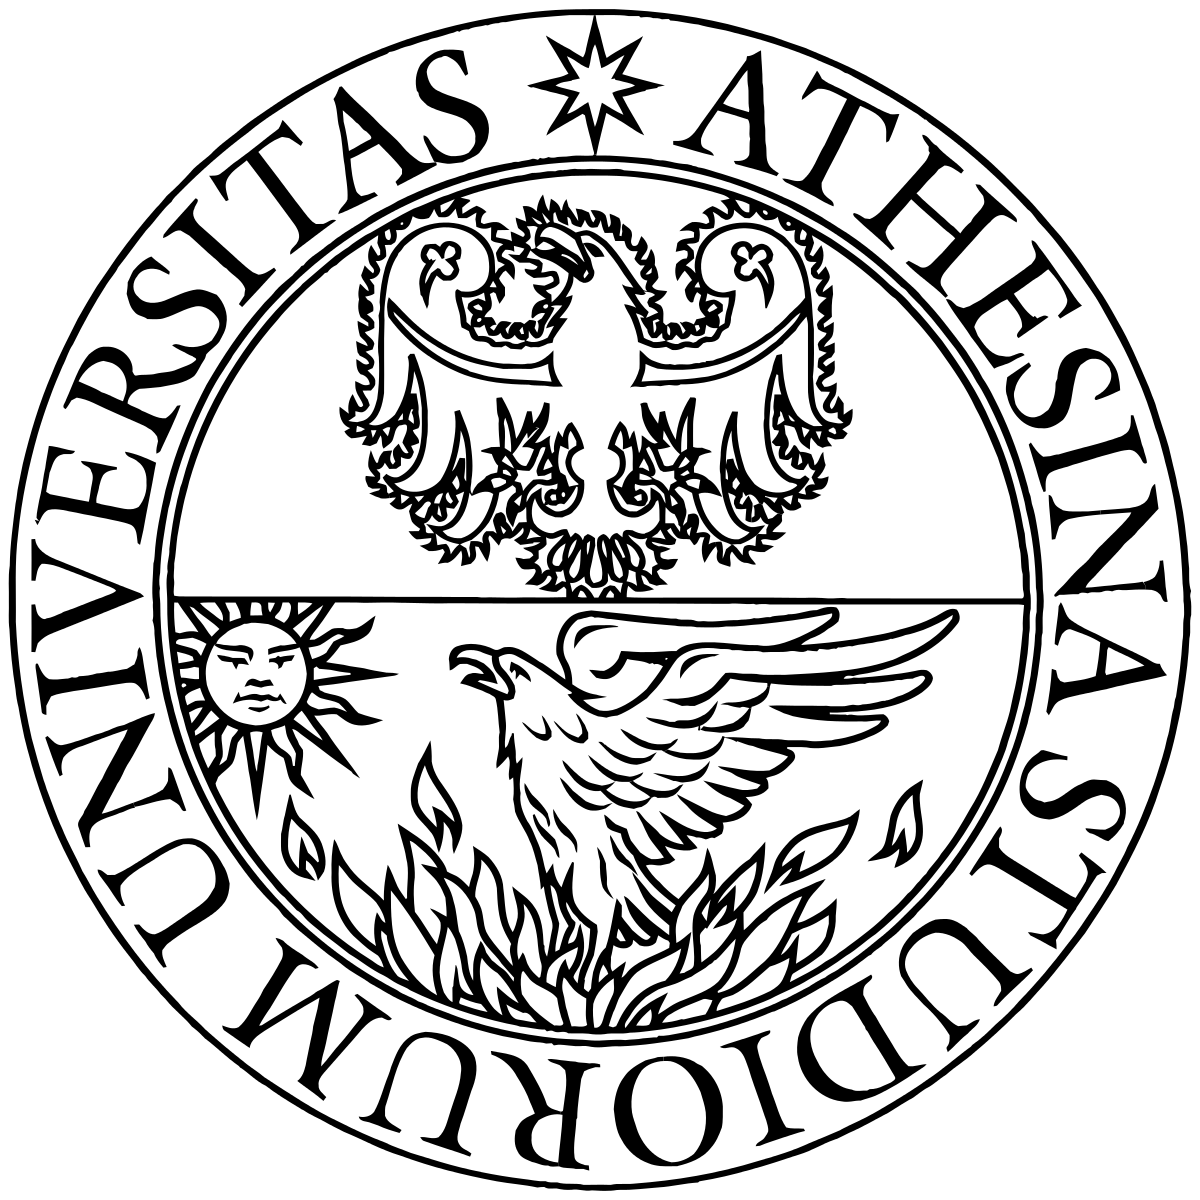
\includegraphics[scale=0.07]{logo.png}\\ 
\end{center}

\maketitle

\begin{center}
    \begin{tabular}{ccc}
    {\bfseries Supervisor:} & \hspace{3cm} {\bfseries Candidate:}\\
    Prof. Francesco Pederiva & \hspace{3cm} Francesco Musso \\
    \end{tabular}
\end{center}

\end{frame}


\section{n-vector model}

\begin{frame}{Lattice models}

\begin{columns}
\column{0.7\textwidth}

\begin{definition}
A \emph{lattice model} is a physical model defined on a discrete space called a 
lattice, a subset of $\mathbb{R}^n$ isomorphic to $\mathbb{Z}^n$, as opposed to 
the continuum of spacetime.
\end{definition}

\vspace{0.5cm}

Introduced in condensed matter physics as atoms in a crystal approximate very
well a lattice. Very useful in computational physics, where discretization of
space become necessary.

\column{0.3\textwidth}
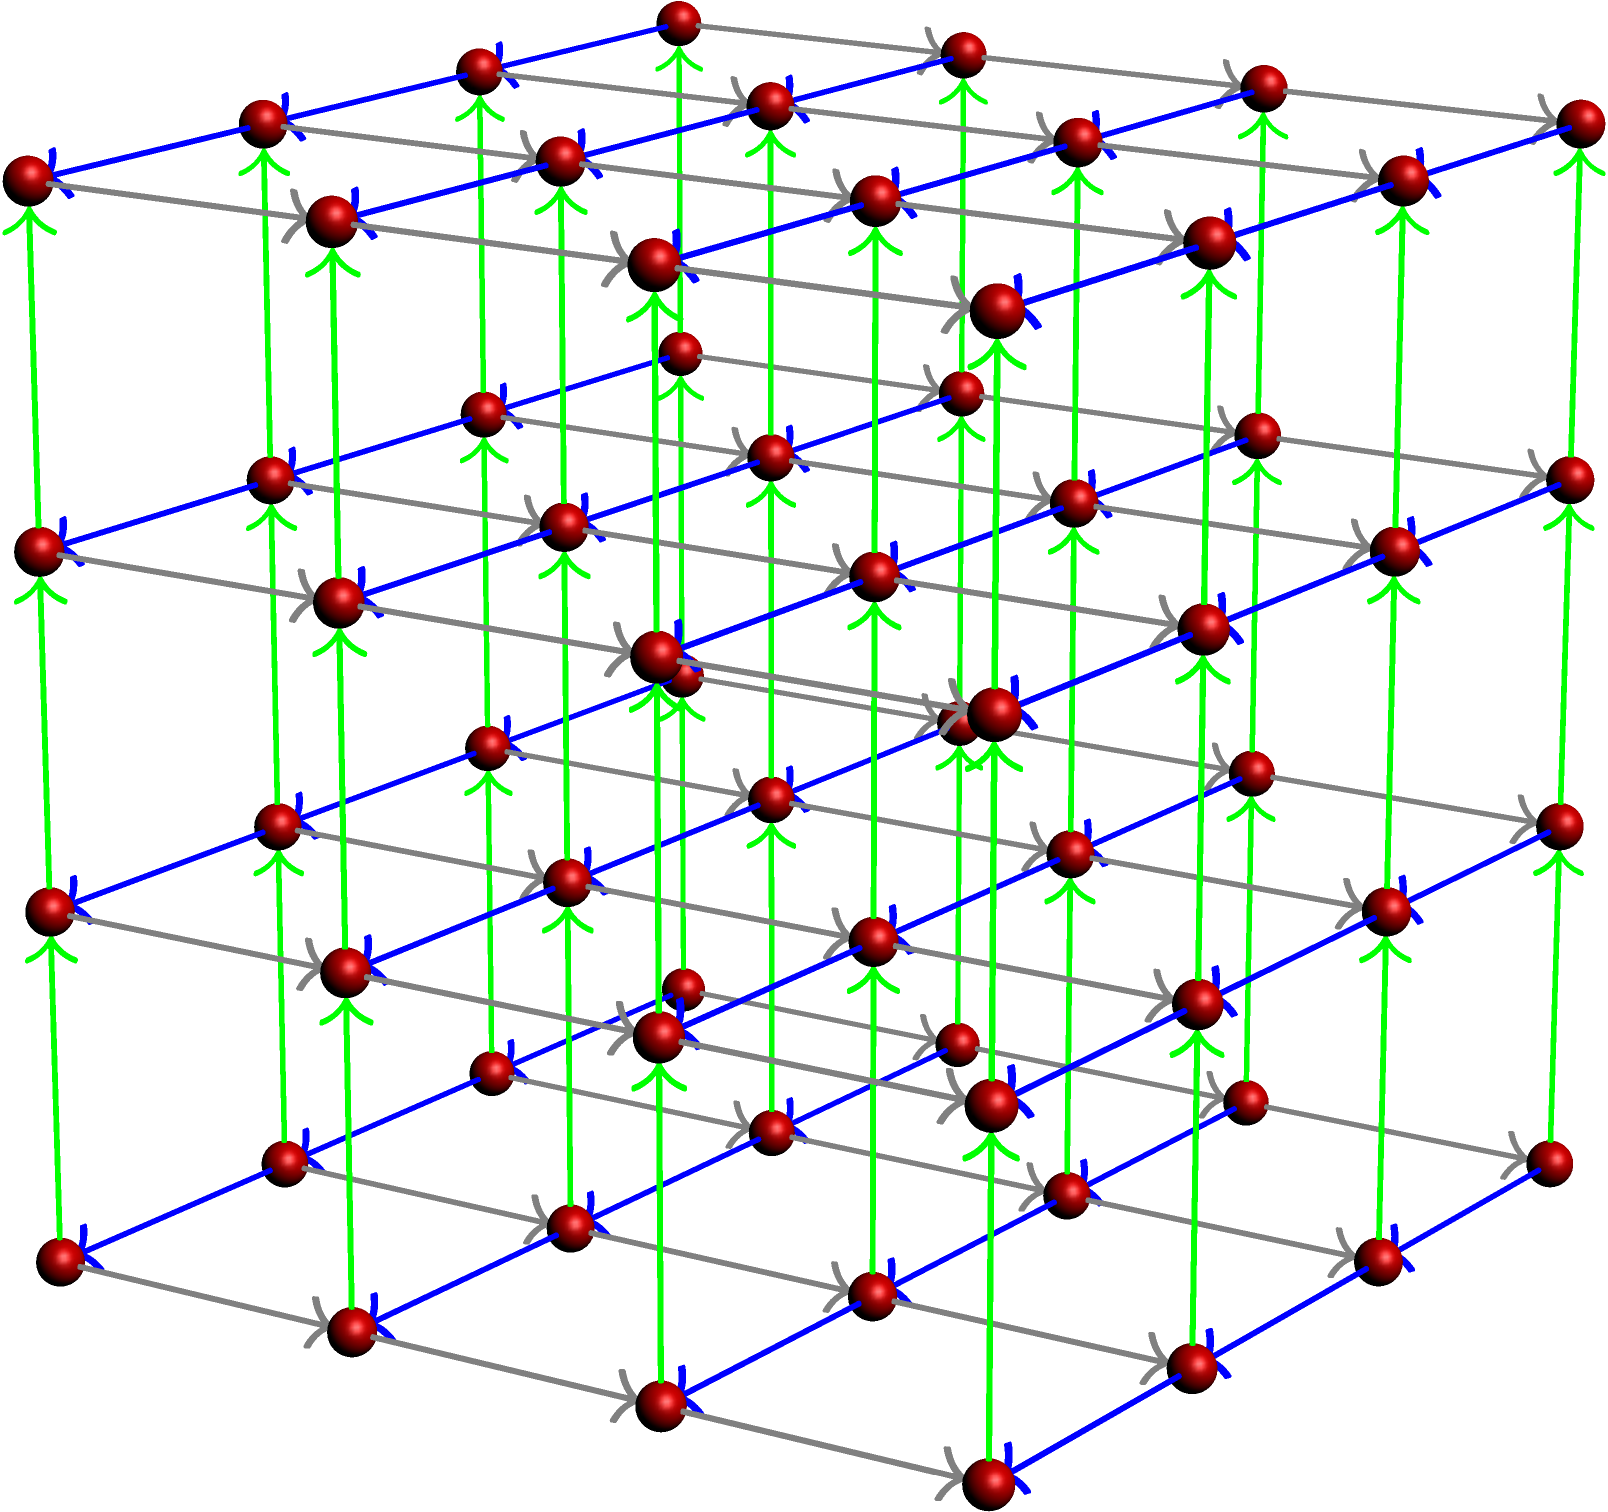
\includegraphics[scale=0.5]{3D_lattice.png}

\end{columns}

\end{frame}


\begin{frame}{n-vector model}

\begin{definition}
A \emph{n-vector model} is a system of spins described by a n-dimensional
unit-lenght vector, located on a lattice site
\end{definition}

\begin{equation}
\boxed{
H = - J \sum_{n.n.} \mathbf{s}_j \cdot \mathbf{s}_i}
\label{eq:ham}
\end{equation}

\begin{itemize}
\item $n=1$ Ising model
\item $n=2$ XY model
\item $n=3$ Heisenberg model
\end{itemize}

\end{frame}


\begin{frame}{Ising model}

\begin{columns}
\column{0.65\textwidth}
From equation~\ref{eq:ham} we can see that the difference between the two possible
configurations of neighbouring spins is
\begin{equation}
\Delta E = E_{\uparrow \uparrow} - E_{\uparrow \downarrow} = -2 J
\end{equation}
then \emph{ferromagnetic} phemonena could arise if $J > 0$, while  
\emph{antiferromagnetic} phenomena could happen if $J < 0$.

\column{0.35\textwidth}
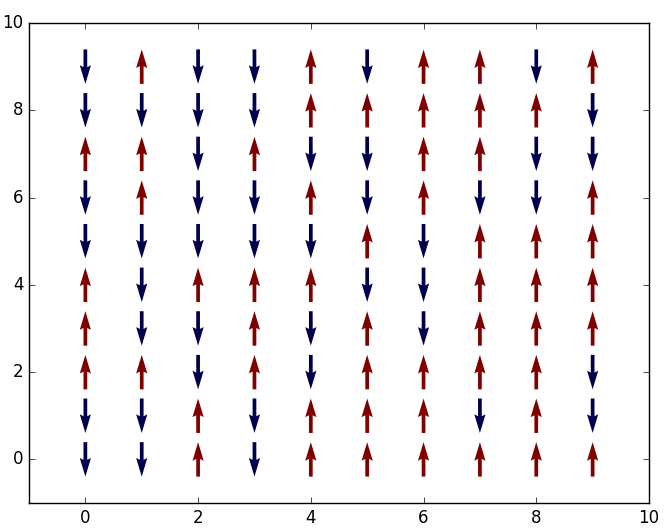
\includegraphics[scale=0.18]{2D_ising.png}

\end{columns}

\vspace{5mm}
Invented much before Stanley's formalization of n-vector models by Wilhelm Lenz.
In 1925 Ising solved the 1D case and showed that no pahse transitions are allowed.

\end{frame}


\section{XY model}

\begin{frame}{2D XY model}

A very interesting case because an infinite-order transition occurs at $k_B T_c /
J \simeq 0.88$: a transition between a quasi-ordered phase at low temperatures and
a disordered phase at high temperatures.

\begin{columns}

\column{0.5\textwidth}
At high temperatures vortices will form, while at $T < T_c$ vortices will try to
annihilate with antivortices. 

\vspace{2mm}

Vortices and antivortices formations are clearly visible in the Monte Carlo
simulation color map of the spin configuration at $k_B T / J = 0.4$ on the right. 

\column{0.5\textwidth}
\centering{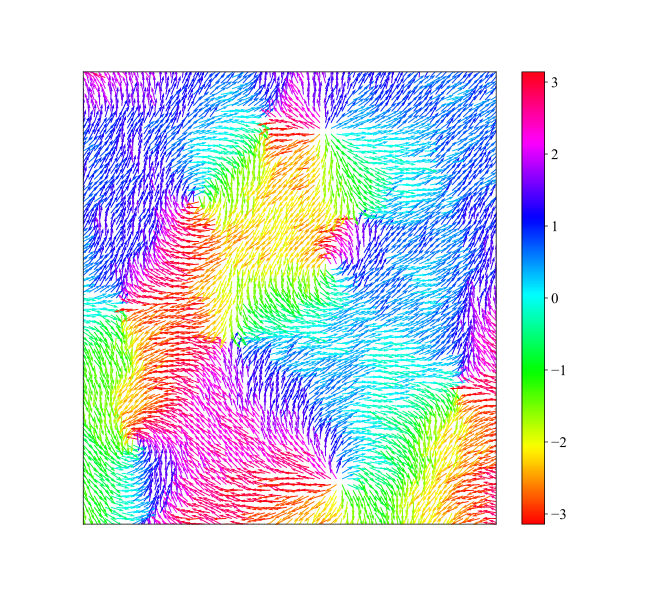
\includegraphics[scale=0.3]{kosterlitz.png}}

\end{columns}
\end{frame}


\begin{frame}{3D XY model}

The most physically interesting situation as experimental data, Monte Carlo
simulation results and theoretical estimates can be compared.

\vspace{5mm}

A ferromagnet-paramagnet phase transition happens at $k_B T_c / J \simeq 2.22$ and 
around this temperature \emph{critical exponents} can be extrapoleted. Critical
exponents are a useful tool to describe the system behaviour around the critical
point.

\end{frame}


\section{Monte Carlo simulations}

\begin{frame}{Monte Carlo simulations}

Used to solve deterministic problems via a probabilistic approach. Based on the
central limit theorem, it's used in dynamical simulation where observables are
averaged over values computed on samples of the system.

\vspace{5mm}

The system configuration is seen as a random variable defined on the phase space,
seen as the sample space. The samples are picked based on the probability
function of the random variable: in this case for example the canonical 
distribution as defined below.

\begin{equation}
P = \frac{\exp(-\beta H)}{Z}
\label{eq:canonical}
\end{equation}
\end{frame}


\begin{frame}{Markov chain sampler}

It is the algorithm which samples the configurations based on the probability
function in equation~\ref{eq:canonical}. Starting from a random configuration
a slightly different one is created and is accepted or not as a new sample
based on the comparison of the probabilities of the two configurations.

\vspace{3mm}

\begin{columns}

\column{0.5\textwidth}
\centering{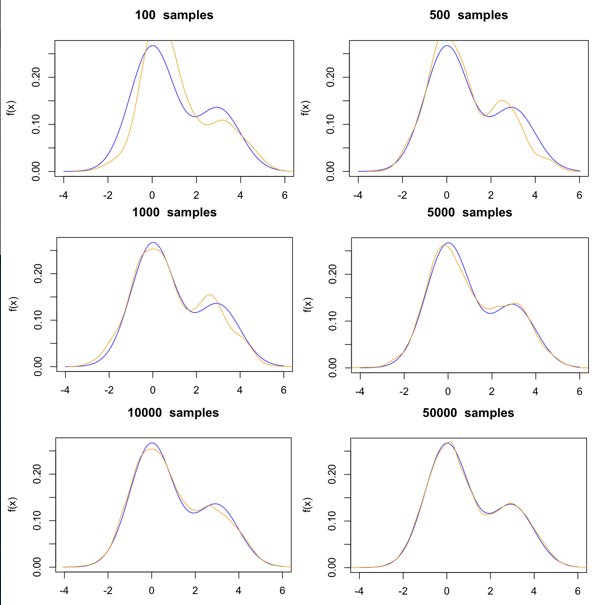
\includegraphics[scale=0.25]{markov.png}}

\column{0.5\textwidth}
Every step is a link in the chain and in the limit of an infinite chain the
samples will approach the probability function as in the figure.

\end{columns}
\end{frame}


\begin{frame}{Metropolis-Hastings algorithm}

Invented in 1953 by Metropolis and Rosenbluth and extended to a more general case
in 1970 by Hastings, is the first Monte Carlo algorithm invented. 

\vspace{3mm}

Being based on the Markov chain sampler it means it violates one of the central 
limit theorem hypothesis: the indipendence of the samples.

\vspace{3mm}

To account for it the Markov chain limit theorem is used which is basically the
same as the original one but it accounts for correlation when estimating the
error on the function value. 

\end{frame}


\section{Results}

\begin{frame}{Implementation}

The Metropolis-Hastings algorithm is used here in the 3D case, on a cube of $L=6$.
Every spin is changed at every step instead of just one, as can be found in most 
of the previous work, to dicrease computational time and correlation.

\vspace{3mm}

The order of magnitude of the change in the angle of the spin is controlled by
$\Delta$ in the following way
\begin{equation}
\theta_i^{\text{mc}} = \theta_i + \Delta (\xi - 0.5)
\end{equation}
where $\xi$ is a random number with uniform distribution in $[0,1]$.

\end{frame}

\begin{frame}

The configurations of interest are the one at equilibrium, then $10\text{k}$ 
inital Monte Carlo steps are dedicated to reach equilibrium and to update the
value of $\Delta$ to reduce correlation. Other $190\text{k}$ steps are executed to
obtain observable values.

\vspace{5mm}

Values of $C_{\text{v}}$ and $M$ where obtained at different temperatures and different
values of the external field $h$. The study is focused on the properties evolution
near the critical point.

\end{frame}

\begin{frame}{Critical exponents}

They are defined as the exponents of the power laws describing the behaviour of 
some physical quantities around the critical temperature. They come from the
assumption that the system is described by an order parameter $m$ that vanishes at
$T_c$.

\vspace{5mm}

So a ordered phase and a disordered phase can be distingiushed: a ordering field
$h$ is then defined as the parameter which opposes the disordering of the system
at high temperature.
\end{frame}


\begin{frame}

It is believed, on strong experimental basis, that they do not depend on the
particular physical system, but only on some of his general properties:
\begin{itemize}
\item the dimensionality of the system
\item the dimensionality of the spin
\item the range of the interaction
\end{itemize}

\vspace{5mm}
In the case of the ferromagnets the parameter $m$ correspond to the magnetization
squared and $h$ to external field.

\vspace{2mm}

An example of a critical exponent could be $\delta$, defined as
\begin{equation}
m \thicksim h^{1/\delta} \quad \text{for}\ T = T_c\ \text{as}\ h \rightarrow 0
\end{equation}

\end{frame}


\begin{frame}{Results}

\begin{columns}

\column{0.5\textwidth}

Graphs of $C_{\text{v}}$ and $M^2$ in respect of $T$, with $h=0$ are reported. The specific
heat has a divergence around $k_B T_c / J \simeq 2.22$ as expected, while for 
$T > T_c$ the magnetization fades rapidly off.

\vspace{5mm}

Fluctuations in the region of $T < T_c$ are due to the fact that the system tends
to jump between states which are local minima of the system, so the system is
stuck in some local minima for quite few steps. 

\column{0.5\textwidth}

\centering{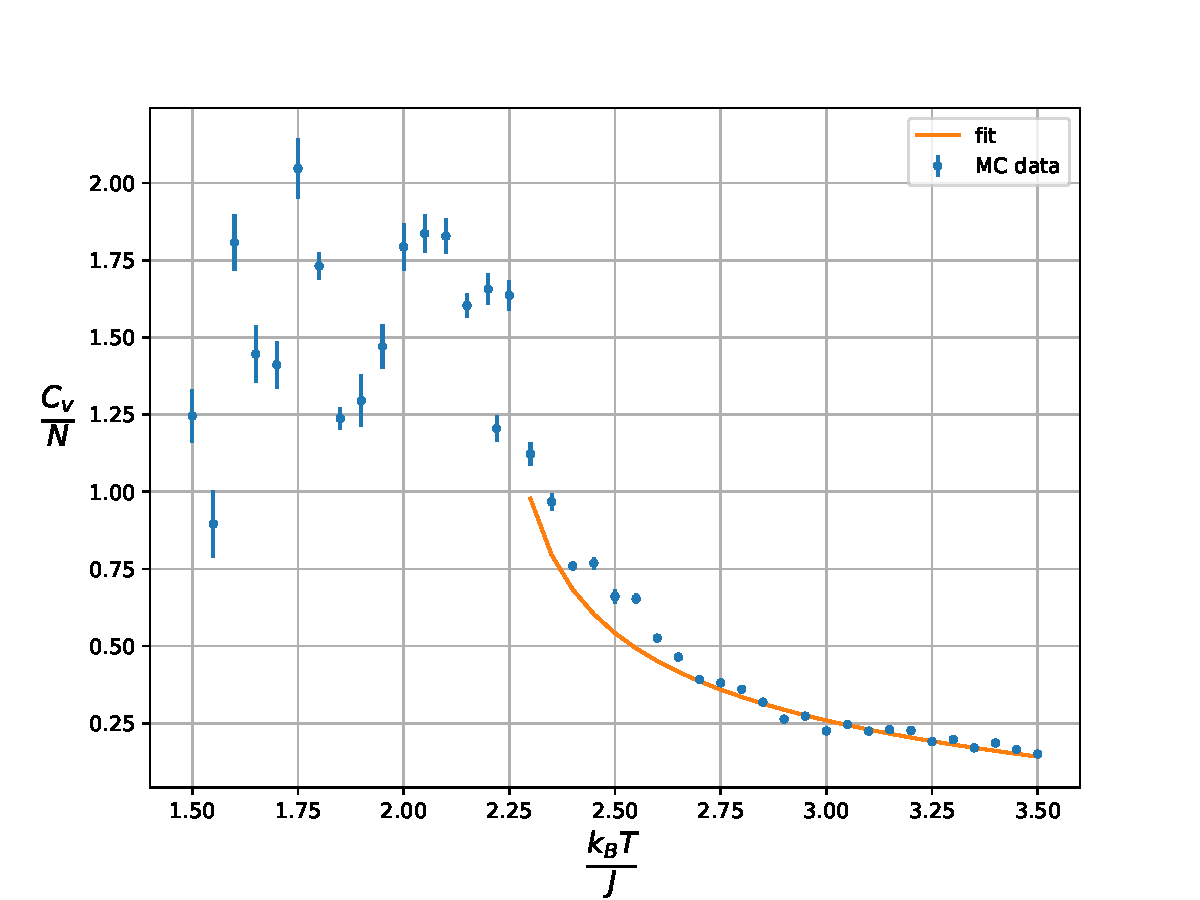
\includegraphics[scale=0.25,page=1]{multipage.pdf}}
\centering{\includegraphics[scale=0.25,page=3]{multipage.pdf}}

\end{columns}
\end{frame}


\begin{frame}

The presence of the ordering field $h$ tends to keep order in the system, above or
below the critical temperature: the fluctuations in energy decrease for $T < T_c$
and magnetization do not vanish immidiately after the critical point. Graphs for
different values of $h$ are reported below.

\vspace{5mm}

\begin{columns}

\column{0.5\textwidth}
\centering{\includegraphics[scale=0.3,page=2]{multipage.pdf}}

\column{0.5\textwidth}
\centering{\includegraphics[scale=0.3,page=4]{multipage.pdf}}

\end{columns}
\end{frame}


\begin{frame}

\begin{columns}

\column{0.5\textwidth}

A study of the magnetization at $T=T_c$ has been carried to extrapolate the
critical exponet $\delta$. The result are reported in the graph on the right.

\vspace{2mm}

Every critical exponent obtained is reported below in the table. Theoretical and
experimental values coming from prevoius works are also reported.

\column{0.5\textwidth}
\centering{\includegraphics[scale=0.3,page=5]{multipage.pdf}}

\end{columns}

\begin{table}[h]
\resizebox{\textwidth}{!}{
\begin{tabular}{|c|c|c|c|c|c|}
\hline
& $\alpha$ & $\beta$ & $\delta$ & $\gamma$ & $\nu$ \\ \hline
Theorical values &  & $0.362 \pm 0.012$ & $4.82 \pm 0.12$ & $1.39 \pm 0.01$ & $0.705 \pm 0.005$ \\ \hline
Experimental values & 0.0-0.2 & 0.3-0.36 & 4.2-4.8 & 1.0-1.2 & 0.62-0.68 \\ \hline
Monte Carlo simulation & $0.201 \pm 0.004$ & $0.438 \pm 0.001$ & $3.86 \pm 0.09$ & $1.08 \pm 0.03$ & $0.654 \pm 0.008$ \\ \hline
$\chi^2_r$ & $\simeq 7\cdot 10^5$ & $\simeq 1\cdot 10^{12}$ & $\simeq 3 \cdot 10^{12}$   &  &    \\ \hline
\end{tabular}}
\end{table}

\end{frame}


\begin{frame}{Possible improvements}

The simulation is not very accurate near and under the critical point. That is a 
known fact and varoius techniques can be used to avoid it.

\vspace{5mm}

The two major issues are the fluctuation in energy and the presence of local
minima of the Hamiltonian near the critical point. They both make the averaging
over the step values much less efficient. 

\vspace{5mm}

Also the fitting function for the critical exponents can be improved by a method
called finite-size scaling.
\end{frame}

\end{document}
